\PassOptionsToPackage{table}{xcolor}
\documentclass[12pt,notheorems]{beamer}
\usetheme{Pittsburgh}
\usepackage[spanish, es-tabla]{babel}
\usepackage[utf8]{inputenc}

\usepackage{amsmath}
\usepackage{amsfonts}
\usepackage{amssymb}
\usepackage[makeroom]{cancel} % Cancel math
%\usepackage{caption} % Caption setup
%\captionsetup{skip=0pt,belowskip=0pt}

\setbeamercovered{transparent} 
\setbeamertemplate{navigation symbols}{} 
\setbeamertemplate{footline}[frame number]
\setbeamertemplate{caption}[numbered]
\usefonttheme[onlymath]{serif}


\usepackage{graphicx} % include figures
\usepackage{hyperref} % With links
\usepackage[table]{xcolor} % pretty tables
\usepackage{booktabs} % Table toprule middlerule bottomrule

\usepackage[group-separator={.}]{siunitx} % point for thousand

\newtheorem{definition}{Definición} % Definition with section numbering
\newtheorem{problem}{Problema} % Definition with section numbering

\setbeamertemplate{frametitle}[default][left]
\setbeamerfont{footnote}{size=\tiny}
\setbeamertemplate{itemize/enumerate body begin}{\footnotesize}
\setbeamertemplate{itemize/enumerate subbody begin}{\tiny}
\setbeamerfont{caption}{size=\footnotesize}


\newcommand{\backupbegin}{
   \newcounter{finalframe}
   \setcounter{finalframe}{\value{framenumber}}
}
\newcommand{\backupend}{
   \setcounter{framenumber}{\value{finalframe}}
}

\author{Felipe A. Glaría Grego}
\title{Diseño e implementación de método de compresión de grafos basados en clustering de cliques maximales}
\subtitle{Defensa de Tesis}
%\logo{
\includegraphics[height=1.5cm]{escudo.png}} 
\institute{
\includegraphics[height=1.5cm]{img/escudo.png}\\Lilian Salinas, Ceciclia Hernández\\Departamento de Ingeniería Informática y Ciencias de la Computación\\Facultad de Ingeniería\\Universidad de Concepción} 
%\date{} 

%\subject{} 
\begin{document}

%\maketitle
\begin{frame}[plain]
\titlepage
\end{frame}

%\begin{frame}
%\tableofcontents
%\end{frame}

\begin{frame}{•}
\frametitle{Motivación}

Gran crecimiento en grafos de redes sociales y de la web.
\begin{itemize}
	\item Estimación sitios indexados: 4,46 mil millones\footnote{\url{http://www.worldwidewebsize.com/}, consultado el 05 de octubre del 2018.}.
	\item Usuarios activos diarios en Facebook: 1,47 mil millones. Crecimiento de 11\% anual\footnote{\href{https://investor.fb.com/investor-news/press-release-details/2018/Facebook-Reports-Second-Quarter-2018-Results/default.aspx}{\texttt{https://investor.fb.com}}, informe de resultados del segundo trimestre del 2018.}.
\end{itemize}

{\parskip=4pt Los grafos de redes sociales son menos comprimibles.
Muy útil descubir usuarios reelevantes y cómo se relacionan, para mejorar resultados de búsquedas, recomendaciones, marketing, entre otros.

Alto costo en recursos que demanda su procesamiento.}
\begin{itemize}
	\item Principalmente espacio en memoria.
	\item Jerarquía de memoria penaliza tiempo de acceso a datos alejados de unidades de procesamiento.
\end{itemize}

\end{frame}


%Principales Soluciones propuestas por otros.
\begin{frame}{•}
\frametitle{Trabajos Relacionados}

{\small
\textbf{WebGraph}, {\footnotesize \textit{Boldi} y \textit{Vigna} (2003)}.

\textbf{k2-tree}, {\footnotesize \textit{Brisaboa}, \textit{Ladra} y \textit{Navarro} (2009)}.

\textbf{Graph Compression by BFS}, {\footnotesize \textit{Apostolico} y \textit{Drovandi} (2009)}.

\textbf{Layered Label Propagation}, de \textit{Boldi}, \textit{Vigna}, \textit{Santini} y \textit{Rosa} (2011).

\textbf{Tight and simple Web graph compression}, {\footnotesize \textit{Grabowski} y \textit{Bieniecki} (2011)}.

\textbf{Compressed representations for web and social graphs}, {\footnotesize \textit{Hernández} y \textit{Navarro} (2014)}.

\textbf{Compressing graphs by grammars}, {\footnotesize \textit{Maneth} y \textit{Peternek} (2016)}.
}

\end{frame}


\begin{frame}
\frametitle{Marco teórico}

\begin{itemize}
	\item Un \textbf{grafo} $G = (V, E)$ como el conjunto finito de \textit{vértices} $V$ (nodos) y el conjunto de \textit{aristas} $E \subseteq V \times V$ (arcos).
	\item Dos vértices $v_{1}$ y $v_{2} \in V(G)$ son \textbf{adyacentes} o \textbf{vecinos} si $(v_{1}, v_{2}) \in E(G)$ y $v_{1} \neq v_{2}$.
	\item Un grafo es \textbf{no dirigido} cuando la arista conlleva ambos sentidos, es decir $(v_{1}, v_{2}) = (v_{2}, v_{1})$.
	\item El \textbf{grado de un vértice} $d(v)$ es la cantidad de vértices en $V(G)$ que son adyacentes con $v$.
	\item La \textbf{matriz de adyacencia} de un grafo $G$ corresponde a una matriz binaria cuadrada $|V(G)| \times |V(G)|$ donde cada bit representa si un par de vértices $v_{1}$ y $v_{2} \in V(G)$ son vecinos o no.
\end{itemize}

\end{frame}



\begin{frame}
\frametitle{Marco teórico (2)}

\begin{itemize}
	\item Un grafo \textbf{k-degenerate} es no dirigido, donde cada subgrafo tiene un vértice con grado a lo más \textbf{k}. 
	\item El índice de \textbf{degeneracy} de un grafo, $D(G)$, es el menor valor \textbf{k} para el cual el grafo es \textbf{k-degenerate}.
	\item Un \textbf{clique} es un subgrafo donde todos los vértices son adyacentes entre sí. Un \textbf{clique maximal} no es subconjunto de otro clique más grande.
	\begin{figure}
    	\centering
    	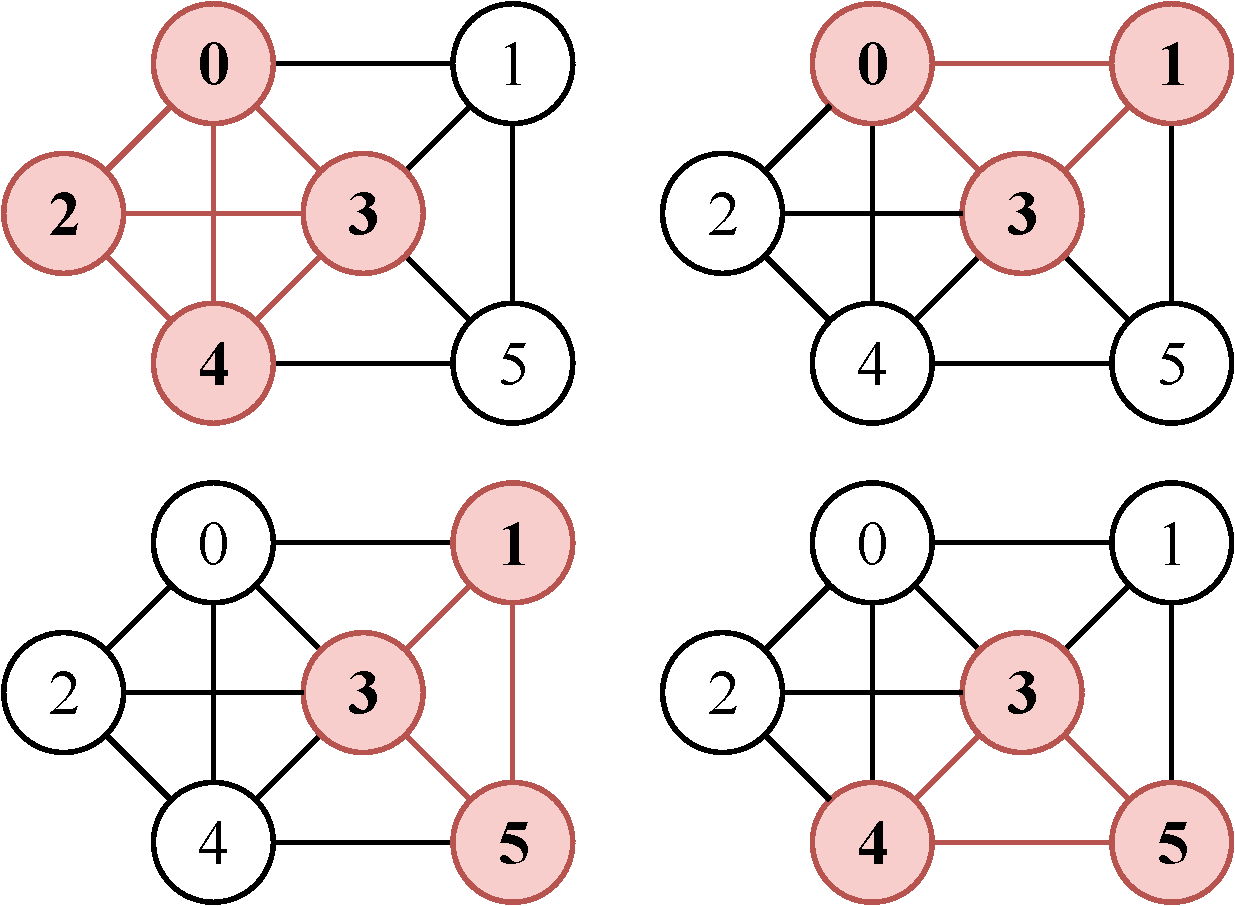
\includegraphics[width=0.4\linewidth]{../img/maxCliqueExample.pdf}
    	
    \caption{Ejemplo de grafo y sus cliques maximales.}
    \label{fig:maxCliqueExample}
\end{figure}
\end{itemize}

\end{frame}


\begin{frame}
\frametitle{Marco teórico (3)}

\begin{itemize}
	\item Un \textbf{triángulo} es un subgrafo de tres vértices y tres aristas. Se define $\lambda(v)$ como la cantidad de triángulos donde participa un nodo $v$.
	\item Se define $\lambda(G)$ como la cantidad de triángulos de un grafo. Se calcula sumando $\lambda(v)$ para cada vértice $v$, y dividiendo el total en tres.
	\begin{equation}
		\lambda(G) = \dfrac{1}{3} \sum_{v \in V} \lambda(v) \label{eq:triangles}
	\end{equation}
	
	\item Un \textbf{triplete} es un subgrafo de tres vértices y dos aristas, donde las aristas comparten un vértice común. Se define $\tau(v)$ como la cantidad de tripletes donde $v$ es el vértice común.
	\item Se define $\tau(G)$ como la cantidad de tripletes de un grafo.
	\begin{equation}
		\tau(G) = \sum_{v \in V} \tau(v) \label{eq:triplets}
	\end{equation}
\end{itemize}

\end{frame}

\begin{frame}
\frametitle{Marco teórico (4)}

\begin{itemize}
	\item El \textbf{coeficiente de clusterización} de un vértice indica cuánto está conectado con sus vecinos, y se define como $c(v) =  \lambda(v) / \tau(v)$. 
	\item El coeficiente de clusterización de un grafo ($C(G)$) es el promedio del coeficiente de todos los nodos del grafo.
	\begin{equation}
		C(G) = \dfrac{1}{|V'|} \sum_{v \in V'} c(v)\label{eq:CC}
	\end{equation}
	con $V' = \{ v \in V | d(v) \geq 2 \}$.
	
	\item La \textbf{transitividad} de un grafo ($T(G)$) es la probabilidad que un par de nodos adyacentes estén interconectados.
	\begin{equation}
		T(G) = \dfrac{3 \lambda(G)}{\tau(G)} \label{eq:T} 
	\end{equation}
\end{itemize}

\end{frame}


%\input{hipotesis}

%% CLIQUES
\begin{frame}
\frametitle{Método de Compresión Propuesto}

Consta de tres etapas:

\begin{enumerate}
	\item Listar todos los cliques maximales del grafo.
	\item Particionar listado de cliques, utilizando heurística eficiente que explote su superposición.
	\item Comprimir particiones en estructura compacta.
\end{enumerate}

\end{frame}


%\begin{frame}
%\frametitle{Etapa 1: Cliques Maximales}
%
%Se obtiene el listado de cliques, usando \textbf{Quick Cliques}\footnote{\url{https://github.com/darrenstrash/quick-cliques}}.
%
%\begin{definition} 
%	\label{def:cliqueGraph}
%	Gafo de cliques
%	
%	Dado un grafo $G = (V, E)$ y $\mathcal{C} = \{c_{1}, c_{2}, ..., c_{N} \}$ el conjunto de tamaño $N$ de cliques maximales que cubren $G$, se tiene $CG_{\mathcal{C}} = (V_{\mathcal{C}}, E_{\mathcal{C}})$ un grafo de cliques donde:
%	
%	\begin{enumerate}
%		\item $V_{\mathcal{C}} = \mathcal{C}$
%		\item $\forall c, c' \in \mathcal{C}, (c, c') \in E_{\mathcal{C}} \Longleftrightarrow c \cap c' \neq \varnothing$
%	\end{enumerate}
%\end{definition}
%
%\end{frame}


\begin{frame}
\frametitle{Etapa 1: Cliques Maximales}

Se obtiene el listado de cliques, usando \textbf{Quick Cliques}\footnote{\url{https://github.com/darrenstrash/quick-cliques}}.

\begin{figure}
    	\centering
    	\begin{minipage}{0.45\textwidth}
    		\centering
    		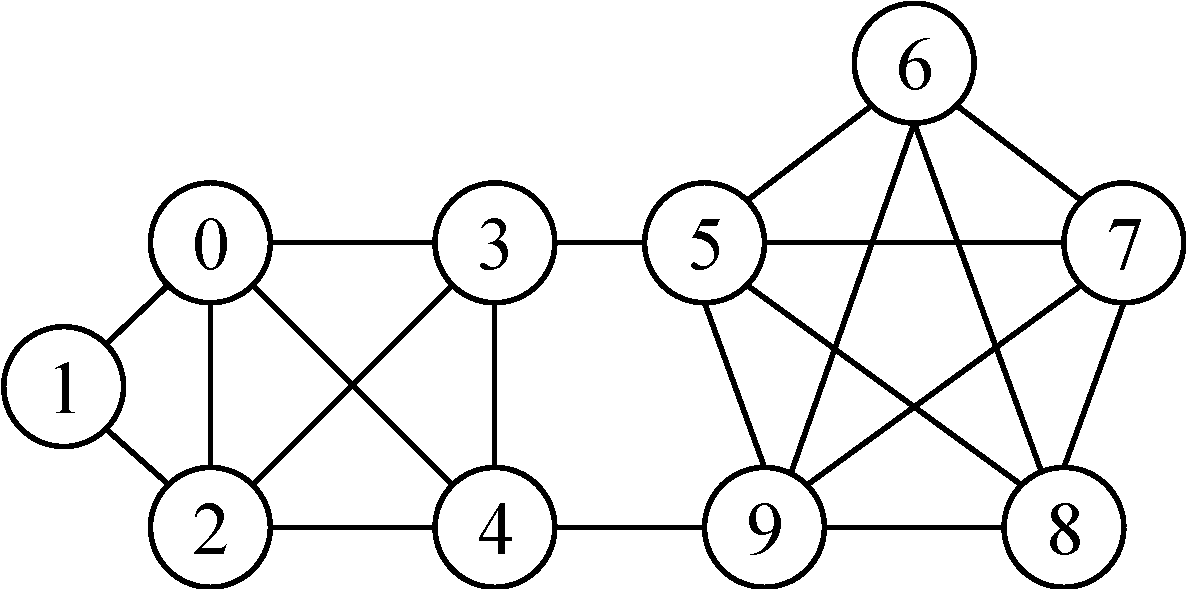
\includegraphics[width=1\linewidth,clip=true]{../img/graphs-Graph2.pdf}
    		(a)
    	\end{minipage}
    	\begin{minipage}{0.25\textwidth}
    		\centering
    		\[
	\begin{aligned}[t]
		C_{0} &: 0, 1, 2 \\
		C_{1} &: 0, 2, 3, 4 \\
		C_{2} &: 3, 5 \\
		C_{3} &: 5, 6, 7, 8, 9 \\
		C_{4} &: 4, 9
	\end{aligned}
\]

    		(b)
    	\end{minipage}
    	\begin{minipage}{0.15\textwidth}
    		\centering
    		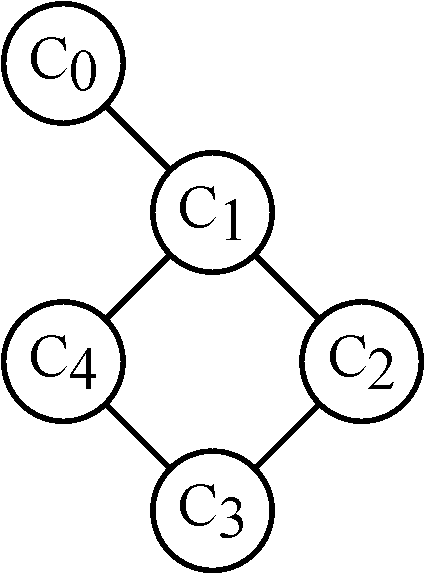
\includegraphics[width=1\linewidth,clip=true]{../img/graphs-Cliques2.pdf}
    		(c)
    	\end{minipage}
    \caption{(a) Grafo no dirigido. (b) Lista de cliques maximales. (c) Grafo de cliques.}
    \label{fig:gafoEj}
\end{figure}

\end{frame}



%% PARTICIONAR
\begin{frame}
\frametitle{Etapa 2: Particionar listado de cliques}

\begin{problem}
	\label{def:findPartitions}
	Encontrar particiones de cliques para el grafo de cliques $CG_{\mathcal{C}}$.
	
	Dado un grafo de cliques $CG_{\mathcal{C}} = (V_{\mathcal{C}}, E_{\mathcal{C}})$, encontrar un set de particiones de cliques $\mathcal{C}\mathcal{P} = \{cp_{1}, cp_{2}, ..., cp_{M}\}$ de $CG_{\mathcal{C}}(V_{\mathcal{C}}, E_{\mathcal{C}})$ con $M \geq 1$, tal que
	\begin{enumerate}
		%\item $\bigcup_{i \in \mathcal{C}\mathcal{P}} cp_{i} = CG_{i}$ \label{item:particiones1}
		\item $\bigcup\limits_{i = 1}^{M} cp_{i} = CG_{\mathcal{C}}$ \label{item:particiones1}
		\item $cp_{i} \cap cp_{j} = \varnothing$ para $i \neq j$ \label{item:particiones2}
		\item cualquier $cp_{i} \in \mathcal{C}\mathcal{P}$ es un subgrafo de $CG_{\mathcal{C}}(V_{\mathcal{C}}, E_{\mathcal{C}})$ inducido por el subset de vértices en $cp_{i}$ \label{item:particiones3}
	\end{enumerate}
	
\end{problem}

\end{frame}


\begin{frame}
\frametitle{Etapa 2: Algoritmo de particionamiento}

Definir una heurística que permita agrupar los cliques en particiones eficientes, que exploten su redundancia de vértices.

\begin{definition} 
	\label{def:rankingFunctions}
	Función de ranking
	
	Dado un grafo $G = (V, E)$ y $\mathcal{C} = \{c_{1}, c_{2}, ..., c_{N} \}$ el conjunto de tamaño $N$ de cliques maximales que cubren $G$, una función de ranking es una función $r: V \rightarrow \mathbb{R}^{+}$ que retorna un valor de puntuación para cada vértice $v \in V$.
\end{definition}

\end{frame}


\begin{frame}
\frametitle{Etapa 2: Algoritmo de particionamiento (2)}

Funciones de ranking propuestas, para $C(u) = \{c \in \mathcal{C}|u \in c\}$:

\begin{align}
	r_{f}(u) &= |C(u)| \label{eq:rankFunF}  \\ 
	r_{c}(u) &= \sum_{c \in C(u)}|c| \label{eq:rankFunC} \\ 
	r_{r}(u) &= \frac{r_{c}(u)}{r_{f}(u)} \label{eq:rankFunR}
\end{align}

%Complejidad: $O(L \log L)$; $L=\sum_{c_i \in \mathcal{C}}|c_{i}|$

\end{frame}


\begin{frame}
\frametitle{Etapa 2: Algoritmo de particionamiento (3)}

\begin{figure}
    	\centering
    	
    	\begin{minipage}{\textwidth}
    		\footnotesize
    		\centering
    		\[
	\begin{aligned}[t]
		C_{0} &: 0, 1, 2 \\
		C_{1} &: 0, 2, 3, 4 \\
		C_{2} &: 3, 5 \\
		C_{3} &: 5, 6, 7, 8, 9 \\
		C_{4} &: 4, 9
	\end{aligned}
\]

    	\end{minipage}
    	
    	\vspace{2mm}
    \begin{minipage}{\textwidth}
    		\footnotesize
    		\centering
    		\begin{tabular}{c|c|c|c|c|c|c|c|c|c|c|}
	\cline{2-11}
	$u \in G$ & 0 & 1 & 2 & 3 & 4 & 5 & 6 & 7 & 8 & 9 \\
	\cline{2-11}
	$R_{rf}$ & 2,0 & 1,0 & 2,0 & 2,0 & 2,0 & 1,0 & 1,0 & 1,0 & 1,0 & 2,0 \\
	\cline{2-11}
	$R_{rc}$ & 7,0 & 3,0 & 7,0 & 6,0 & 6,0 & 7,0 & 5,0 & 5,0 & 5,0 & 7,0 \\
	\cline{2-11}
	$R_{rr}$ & 3,5 & 3,0 & 3,5 & 3,0 & 3,0 & 3,5 & 5,0 & 5,0 & 5,0 & 3,5 \\
    \cline{2-11}
\end{tabular}

    \end{minipage}
    
    	\caption{Listado de cliques y puntajes de ranking asociados.}
    \label{fig:rankings}
\end{figure}

\end{frame}



\begin{frame}
\frametitle{Etapa 2: Algoritmo de particionamiento (4)}

\begin{algorithm}[H]
\caption{\footnotesize Algoritmo de particionamiento del grafo de cliques.}
\begin{algorithmic}[1]
\scriptsize
\REQUIRE $\mathcal{C}$ maximal clique collection ($N=|\mathcal{C}|$), ranking function $r(u)$
\ENSURE Returns clique-graph partition collection $\mathcal{C}\mathcal{P}$
\STATE $(D,R) \leftarrow computeRanking(r,\mathcal{C})$ (array $D$ y $R$, $\forall u \in V$ ) \label{alg:clustering:rankarray} 
\STATE Initialize bit array $Z$ of size $N$ and set each bit to 0
\FOR {$u \in R$}
    \STATE $cpid \leftarrow \emptyset$
     \FOR {$id \in D[u]$ and $Z[id]=0$} 
          \STATE $Z[id] \leftarrow 1$
          \STATE $cpid \leftarrow cpid \cup \{id\}$
    \ENDFOR
    \IF {$cpid \neq  \emptyset$}
      \STATE $\mathcal{C}\mathcal{P} \leftarrow \mathcal{C}\mathcal{P} : cpid$
    \ENDIF 
 \ENDFOR
\RETURN $\mathcal{C}\mathcal{P}$
\end{algorithmic}
\end{algorithm}

Complejidad: $O(N+V)$

\end{frame}		



\begin{frame}
\frametitle{Etapa 2: Algoritmo de particionamiento (5)}

\begin{figure}
    	\centering
    	
    	\begin{minipage}{\textwidth}
    		\footnotesize
    		\centering
    		\[
	\begin{aligned}[t]
		C_{0} &: 0, 1, 2 \\
		C_{1} &: 0, 2, 3, 4 \\
		C_{2} &: 3, 5 \\
		C_{3} &: 5, 6, 7, 8, 9 \\
		C_{4} &: 4, 9
	\end{aligned}
\]

    	\end{minipage}
    	
    	\vspace{2mm}
    	\begin{minipage}{\textwidth}
    		\footnotesize
    		\centering
    		\begin{tabular}{c|c|c|c|c|c|c|c|c|c|c|}
	\cline{2-11}
	$u \in G$ & 0 & 1 & 2 & 3 & 4 & 5 & 6 & 7 & 8 & 9 \\
	\cline{2-11}
	$R_{rf}$ & 2,0 & 1,0 & 2,0 & 2,0 & 2,0 & 1,0 & 1,0 & 1,0 & 1,0 & 2,0 \\
	\cline{2-11}
	$R_{rc}$ & 7,0 & 3,0 & 7,0 & 6,0 & 6,0 & 7,0 & 5,0 & 5,0 & 5,0 & 7,0 \\
	\cline{2-11}
	$R_{rr}$ & 3,5 & 3,0 & 3,5 & 3,0 & 3,0 & 3,5 & 5,0 & 5,0 & 5,0 & 3,5 \\
    \cline{2-11}
\end{tabular}

    	\end{minipage}
    	
    	\vspace{2mm}
    \begin{minipage}{\textwidth}
    		\footnotesize
    		\centering
    		\begin{tabular}{c|c|c|c|c|}
	\cline{2-5}
	$\mathcal{C}\mathcal{P}_{rf}$ & $C_{0} \quad C_{1}$ & $C_{2}$ & $C_{4}$ & $C_{3}$ \\
	\cline{2-5}
	$\mathcal{C}\mathcal{P}_{rc}$ & $C_{0} \quad C_{1}$ & $C_{2} \quad C_{3}$ & $C_{4}$ \\
	\cline{2-5}
	$\mathcal{C}\mathcal{P}_{rr}$ & $C_{3}$ & $C_{0} \quad C_{1}$ & $C_{2}$ & $C_{4}$ \\
	\cline{2-5}
\end{tabular}

    \end{minipage}
    
    	\caption{Particiones de cliques para cada función de ranking.}
    \label{fig:CPpartitions}
\end{figure}

\end{frame}




%% ESTRUCTURAS COMPACTAS
\begin{frame}
\frametitle{Etapa 3: Estructuras Compactas - Secuencias}

\begin{itemize}
	\item \textbf{X}: Listas concatenadas de vértices en $\mathcal{C}\mathcal{P}$.
	\item \textbf{B}: Bitmap indicando inicio de particiones.
	\item \textbf{BB}: Secuencia de bytes codificando presencia de vértices en cliques por partición.
	\item \textbf{Y}: Secuencia de enteros indicando primer byte en \textbf{BB} para cada partición.
\end{itemize}

\end{frame}


\begin{frame}
\frametitle{Etapa 3: Estructuras Compactas - Secuencias (2)}

\begin{figure}
    	\centering
    	
    	\begin{minipage}{\textwidth}
    		\footnotesize
    		\centering
    		\[
	\begin{aligned}[t]
		C_{0} &: 0, 1, 2 \\
		C_{1} &: 0, 2, 3, 4 \\
		C_{2} &: 3, 5 \\
		C_{3} &: 5, 6, 7, 8, 9 \\
		C_{4} &: 4, 9
	\end{aligned}
\]

    	\end{minipage}
    	
    	\vspace{2mm}
    	\begin{minipage}{\textwidth}
    		\footnotesize
    		\centering
    		\begin{tabular}{c|c|c|c|c|}
	\cline{2-5}
	$\mathcal{C}\mathcal{P}_{rr}$ &  $C_{0} \quad C_{1}$ & $C_{3}$ & $C_{2}$ & $C_{4}$ \\
	\cline{2-5}
\end{tabular}

    	\end{minipage}
    	
    	\vspace{2mm}
    \begin{minipage}{\textwidth}
    		\footnotesize
    		\centering
    		\begin{tabular}{c|c|c|c|c|c|c|c|c|c|c|c|c|c|c|c|}
	\cline{2-15}
	$X$: & 0 & 1 & 2 & 3 & 4 & 5 & 6 & 7 & 8 & 9 & 3 & 5 & 4 & 9 \\
	\cline{2-16}
	$B$: & 1 & 0 & 0 & 0 & 0 & 1 & 0 & 0 & 0 & 0 & 1 & 0 & 1 & 0 & 1 \\
	\cline{2-16}
	$BB$: & 3 & 1 & 3 & 2 & 2 \\
	\cline{2-6}
	$Y$: & 0 & 5 \\
	\cline{2-3}
\end{tabular}

    \end{minipage}
    
    	\caption{Secuencias finales.}
    \label{fig:sequences}
\end{figure}

\end{frame}



% ALGORITMOS
\begin{frame}
\frametitle{Algoritmos de consulta - Reconstrucción secuencial}

Recorre las particiones en orden secuencial.
\begin{itemize}
	\item Si contiene solo un clique, sus vértices son vecinos.
	\item Si no, se comparan los bytes de cada vértice entre si.
		\begin{itemize}
		\footnotesize
		\item Si la comparación es distinto a cero, son vecinos.
		\item No es necesario comparar siguientes bytes.
	\end{itemize}
\end{itemize}

\vspace{6mm}
Complejidad: 
$\begin{cases}
	O(P_{0} \cdot N^{2}), & bpu_{p} = 0 \\
	O(P_{1} \cdot N^{2} \cdot bpu_{p}), & bpu_{p} \neq 0  \\
\end{cases}$

\vspace{3mm}
{\footnotesize
$bpu_{p}$: Bytes por vértice de particiones.

$P_{0}$: Particiones que no tienen bytes por vértice.

$P_{1}$: Particiones que sí tienen bytes por vértice.

$N$: Largo de particiones.
}

\end{frame}


\begin{frame}
\frametitle{Algoritmos de consulta - Listado de vecinos}

Para un vértice $u$ aleatorio.
\begin{itemize}
	\item Cuenta ocurrencias de $u$ en $X$.
	\item Por cada una, se identifica su partición.
	\begin{itemize}
		\footnotesize
		\item Si contiene solo un clique, sus vértices son vecinos de $u$.
		\item Si no, se comparan sus bytes con los de cada posible vecino.
		\begin{itemize}
			\footnotesize
			\item Si la comparación es distinto a cero, son vecinos.
			\item No es necesario comparar siguientes bytes.
		\end{itemize}	
	\end{itemize}
\end{itemize}

\vspace{6mm}
Complejidad: 
$\begin{cases}
	O(M_{0} \cdot N), & bpu_{p} = 0 \\
	O(M_{1} \cdot N \cdot bpu_{p}), & bpu_{p} \neq 0  \\
\end{cases}$

\vspace{3mm}
{\footnotesize
$bpu_{p}$: Bytes por vértice de particiones.

$M_{0}$: Particiones que contienen a $u$ y no tienen bytes por vértice.

$M_{1}$: Particiones que contienen a $u$ y  sí tienen bytes por vértice.

$N$: Largo de particiones.
}

\end{frame}



\begin{frame}
\frametitle{Algoritmos de consulta - Vecindad de dos vértices}

Para dos vértices $u_{1}$, $u_{2}$ aleatorios.
\begin{itemize}
	\item Cuenta ocurrencias de ambos vértices en $X$.
	\item Revisa si coinciden en una partición
	\begin{itemize}
		\footnotesize
		\item Si coinciden, se comparan sus bytes.
		\begin{itemize}
			\footnotesize
			\item Si la comparación es distinto a cero, son vecinos.
			\item No es necesario comparar siguientes bytes.
		\end{itemize}
	\end{itemize}
\end{itemize}

\vspace{6mm}
Complejidad: 
$\begin{cases}
	O(M_{1} + M_{2}), & bpu_{p} = 0 \\
	O((M_{1} + M_{2}) \cdot bpu_{p}), & bpu_{p} \neq 0  \\
\end{cases}$

\vspace{3mm}
{\footnotesize
$bpu_{p}$: Bytes por vértice de particiones.

$M_{1}$: Particiones que contienen a $u_{1}$.

$M_{2}$: Particiones que contienen a $u_{2}$.
}

\end{frame}



\begin{frame}
\frametitle{Algoritmos de consulta - Cliques maximales}

Recorre las particiones en orden secuencial.
\begin{itemize}
	\item Si contiene un solo clique, lista sus vértices.
	\item Si no, se revisan los bytes de cada vértice ordenadamente.
	\begin{itemize}
		\footnotesize
		\item Si comparten un 1 en mismo bit, son un clique.
	\end{itemize}
\end{itemize}

\vspace{6mm}
Complejidad: 
$\begin{cases}
	O(P_{0} \cdot N), & bpu_{p} = 0 \\
	O(P_{1} \cdot N \cdot 8 \cdot bpu_{p}), & bpu_{p} \neq 0  \\
\end{cases}$

\vspace{3mm}
{\footnotesize
$bpu_{p}$: Bytes por vértice de particiones.

$P_{0}$: Particiones que no tienen bytes por vértice.

$P_{1}$: Particiones que sí tienen bytes por vértice.

$N$: Largo de particiones.
}

\end{frame}


%\input{metodologia}

%\input{adelantado}

%\input{planificacion}

{
\setbeamercolor{background canvas}{bg=black}
\begin{frame}[plain]
\centerline{
\includegraphics[]{img/handshakeInv.png}}
\begin{center}
{\Huge \color{white}Muchas gracias}
\end{center}
\end{frame}
}

\appendix
\backupbegin
%\input{anexo/popular}
%\input{anexo/sdsl}
%\input{anexo/similitud}
%\input{anexo/minhash}
\backupend

\end{document}